\documentclass[oneside, a4paper]{article}
\usepackage[utf8]{inputenc}
\usepackage[english]{babel}
\usepackage[hypertexnames=false]{hyperref} 
\hypersetup{
    colorlinks=true,
    linkcolor=black,
    filecolor=magenta,      
    urlcolor=cyan,
}

\urlstyle{same}
\usepackage{textcomp}
\usepackage[utf8]{inputenc}
\usepackage{graphicx}
\usepackage{array}
\usepackage{soul}
\usepackage{amsmath}
\usepackage{forest}
\usepackage{mathtools}
\DeclarePairedDelimiter\ceil{\lceil}{\rceil}
\DeclarePairedDelimiter\floor{\lfloor}{\rfloor}


% Set spacing (i set it to 1.2x)
\renewcommand{\baselinestretch}{1}
% Indentation (set this to zero for normal prose)
\setlength{\parindent}{0em}
% Line breaking (spacing between paragraphs)
\setlength{\parskip}{0.5em}

% Use the whole page
\usepackage{geometry}
% Extra math glyphs
\usepackage{amsmath}
% Proper enumerate spacing
\usepackage{enumitem}
% More pleasing screen fonts
\usepackage{lmodern}
% Fancy headers
\usepackage{fancyhdr}
\usepackage{graphicx}
\usepackage{algpseudocode}
% Allows absolute positioning of images
\usepackage{float}
% \usepackage[section]{placeins}
% Set no separation
\setlist{noitemsep}
% Set margins to reasonable
\geometry{margin=2.5cm}
% Sets graphics path
\graphicspath{ {./images/} }
% Sets up fancy headers

\addto\captionsenglish{
}


\usepackage{listings}
\usepackage{color}

\pagestyle{plain}

\begin{document}


\definecolor{dkgreen}{rgb}{0,0.6,0}
\definecolor{gray}{rgb}{0.5,0.5,0.5}
\definecolor{mauve}{rgb}{0.58,0,0.82}

\lstset{frame=tb,
  language=Java,
  aboveskip=3mm,
  belowskip=3mm,
  showstringspaces=false,
  columns=flexible,
  basicstyle={\small\ttfamily},
  numbers=none,
  numberstyle=\tiny\color{gray},
  keywordstyle=\color{blue},
  commentstyle=\color{dkgreen},
  stringstyle=\color{mauve},
  breaklines=true,
  breakatwhitespace=true,
  tabsize=3
}

\pagestyle{fancy}
\fancyhf{}
\lhead{s4530974 - Homework Assignment 2}
\rhead{COMP3506}

\begin{titlepage}
\newgeometry{left=7.5cm} %defines the geometry for the titlepage
\noindent
\color{black}
\makebox[0pt][l]{\rule{1.3\textwidth}{1pt}}

{\Huge {Student - s4530974}}
\vskip\baselineskip
\noindent
{\huge{COMP3506 - Homework 2}}

\vskip\baselineskip
{\large {Semester 2 - 2020}}
\end{titlepage}

\newpage

\setcounter{secnumdepth}{-1}
\section{Question 2}

\section{Results - Graphs and Tables}
The following results will be shown in tables and graphs. Please note that a lot of the data points were very small and are not visible due to the axis having to stretch across the large input range. The boolean for reversed that I passed into my timed functions was false which slightly influenced my results for the ascending sorted list.

\subsection{Unsorted Order}

\begin{table}[ht]
    \centering
    \caption{Unsorted Order Results Table for Different Sorting Algorithms}
    \begin{tabular}[t]{|l| l l l l l l l|} 
    \hline
    & n = 5 & n = 10 & n = 50 & n = 100 & n = 500 & n = 1000 & n = 10000\\ [0.5ex] 
    \hline
    Selection Sort & 1.1087 &	0.0234 &	0.3089 & 	0.8749 & 	4.7579	& 5.1673 &	73.806  \\ 
    \hline
    Insertion Sort & 0.0007 &	0.0154 &	0.049	 & 0.2743	 & 2.307	& 3.7151 &	73.3882 \\
    \hline
    Merge Sort & 0.0147 &	0.0215 &	0.068	 & 0.1309	 & 0.289	& 0.5076 &	2.0947\\
    \hline
    Quick Sort & 0.0091 &	0.0234 &	0.0324 & 	0.0609 & 	0.363	& 0.1505 &	2.0337 \\
     \hline
    \end{tabular}
\end{table}

\
\begin{figure}[!ht]
	\centerline{\frame{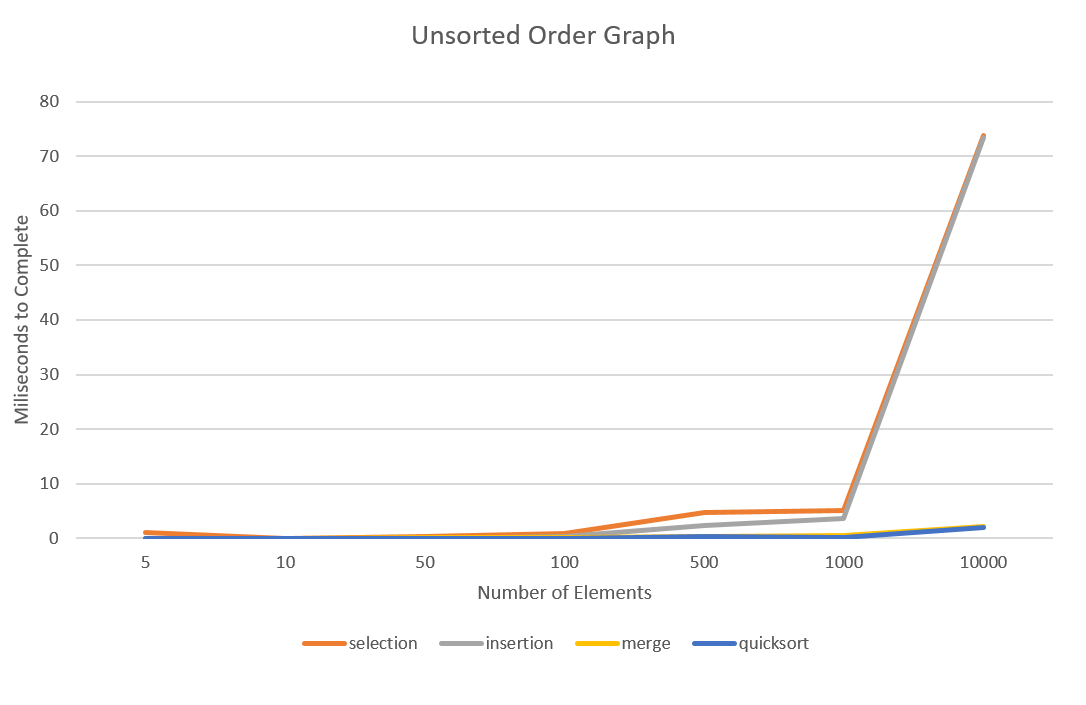
\includegraphics[scale=0.75]{U.png}}}
	\label{fig:figure1}
\end{figure}

\newpage

\subsection{Ascending Order}

\begin{table}[ht]
    \centering
    \caption{Ascending Order Results Table for Different Sorting Algorithms}
    \begin{tabular}[t]{|l| l l l l l l l|} 
    \hline
    & n = 5 & n = 10 & n = 50 & n = 100 & n = 500 & n = 1000 & n = 10000\\ [0.5ex] 
    \hline
    Selection Sort & 0.6688	& 0.3961 &	0.7252 &	0.492	 & 5.393 &	10.2032	& 119.1348 \\ 
    \hline
    Insertion Sort & 0.0083	& 0.0077 &	0.0016 &	0.0081 & 	0.0286	& 0.0708 &	0.4758\\
    \hline
    Merge Sort & 0.0125	& 0.0073 &	0.0107 &	0.0904 & 	0.6185	& 0.3593 &	2.4167\\
    \hline
    Quick Sort & 0.0102	& 0.0043 &	0.0065 &	0.023	 & 0.2813	& 0.1294 &	0.7787 \\
     \hline
    \end{tabular}
\end{table}

\begin{figure}[!ht]
	\centerline{\frame{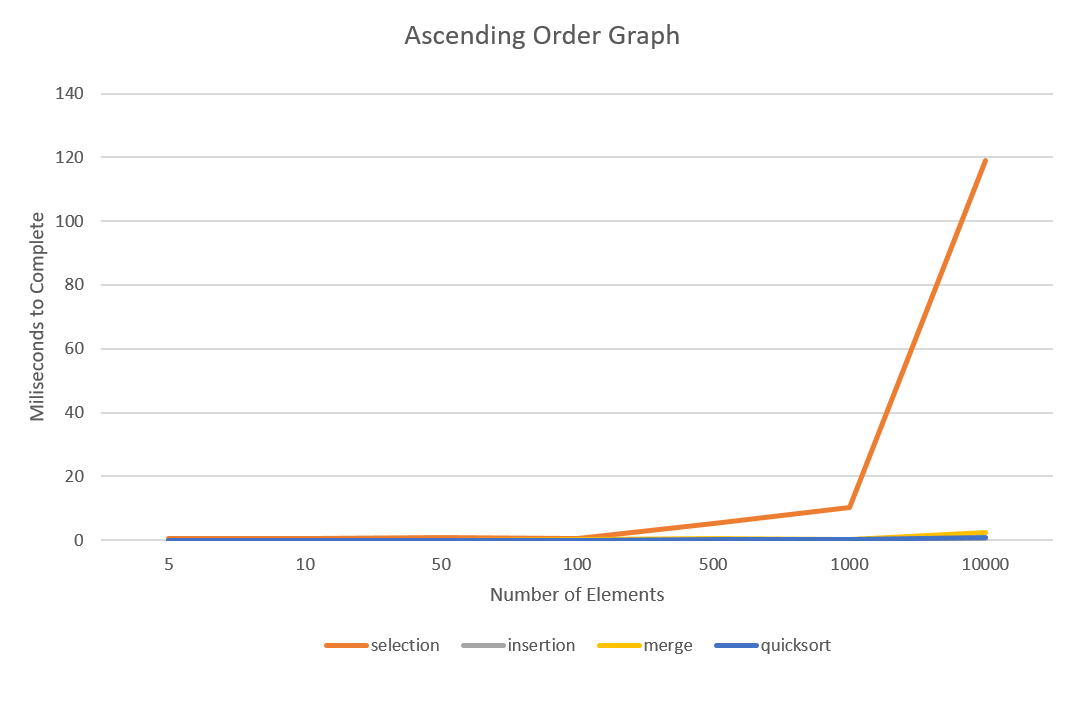
\includegraphics[scale=0.9]{A.png}}}
	\label{fig:figure1}
\end{figure}
\newpage

\subsection{Descending Order}
\begin{table}[ht]
  \centering
  \caption{Descending Order Results Table for Different Sorting Algorithms}
  \begin{tabular}[t]{|l| l l l l l l l|} 
  \hline
  Algorithm & n = 5 & n = 10 & n = 50 & n = 100 & n = 500 & n = 1000 & n = 10000\\ [0.5ex] 
  \hline
  Selection Sort & 1.376 &	0.0074 & 0.1192 & 0.4035 & 4.1453 & 1.1147 & 72.5723 \\ 
  \hline
  Insertion Sort &  0.0049 & 0.0046	& 0.1183	& 0.314 & 	4.4156	& 8.7376	& 199.0831\\
  \hline
  Merge Sort & 0.0075 &	0.0083	& 0.0884	& 0.1255	& 0.5191	& 0.4094	& 1.4769\\
  \hline
  Quick Sort & 0.0059	& 0.0049	& 0.0308	& 0.0599	& 0.1927	& 0.1309	& 0.8572\\
   \hline
  \end{tabular}
\end{table}

\begin{figure}[!ht]
	\centerline{\frame{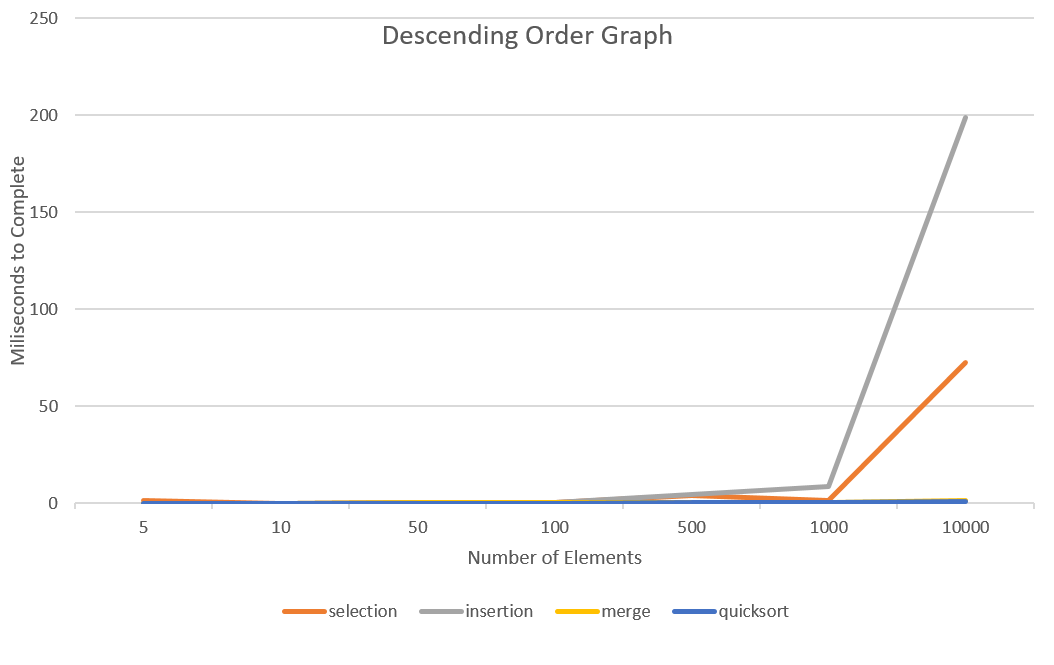
\includegraphics[scale=0.95]{D.png}}}
	\label{fig:figure1}
\end{figure}


\newpage
\section{Results Analysis}
The first thing that I was able to notice was that the Big-$O$ of Selection and Insertion sort is that of $O(n^2)$ meaning that the runtime graphs of the sorts did not change the graph trends for either when the input was changed. Quick sort and merge sort both have a Big-$O$ complexity of expected $O(nlog(n))$ with quicksort having a worst case Big-$O$ of $O(n^2)$. First, it’s worth noting that in comparison to selection and insertion sorts, merge and quick sort have less runtime. Secondly, as the number of inputs increases (500 – 10 000), quick sort and merge sort both increase steadily but not at the same rate as insertion and selection sorts. 

Something that was assumed within the data I received was that the time taken to execute each sorting function would increase with the input size. This was proven to be a correct assumption as all the graphs/tables that I was able to generate have a noticeable increase in time taken per input.

When comparing the ascending input times to the descending input times. It is evident that there was less time spent executing the sort. This was because the elements were sorted in the right order (ascending) meaning that there were less iterations and less time spent going through the array making it faster. 

When looking at the unsorted algorithm time, I was lucky that the worst case for the quick sort algorithm I had was never triggered within the unsorted input which would have resulted in a larger time taken due to the pivots chosen. It’s interesting to note that the times taken for the unsorted input for selection and insertion sort are less than the ascending and descending inputs. This might be an outlier or I might have gotten very lucky with my random inputs.

\section{Written Code}
The way that my timing algorithm worked was utilising System.nanoTime() which wrapped around each sorting algorithm. I would then have 3 separate functions which would create different arrays according to the specifications. Each of these functions would then pass the created array into a function which would time them and print out the time taken to execute each function and looked like the following:

\begin{lstlisting}
import java.awt.desktop.SystemEventListener;
import java.util.Arrays; 
import java.util.Collections;
import java.util.Random;


public class TimedSorting {
    private int[] arraySizes = {5, 10, 50, 100, 500, 1000, 10000};
    Random rand = new Random();

    // Creates a randomised array
    private <T extends Comparable> T[] populateArray(int arraySize) {
        T[] array = (T[]) new Comparable[arraySize];
        for (int i = 0 ; i < arraySize; i++) {
            array[i] = (T)(Integer)rand.nextInt();
        }
        return array;
    }

    // Time the time it takes for each sorting algorithm
    public <T extends Comparable> void timeArray(T[] array) {
        // Selection Sort
        T[] copiedArray = array.clone();
        long startTime = System.nanoTime();
        SortingAlgorithms.selectionSort(copiedArray, false);
        long endTime = System.nanoTime();
        System.out.println("Selection Sort," + ((endTime - startTime)/1000000.0));

        // Insertion Sort
        copiedArray = array.clone();
        startTime = System.nanoTime();
        SortingAlgorithms.insertionSort(copiedArray, false);
        endTime = System.nanoTime();
        System.out.println("Insertion Sort," + ((endTime - startTime)/1000000.0));

        // Merge Sort
        copiedArray = array.clone();
        startTime = System.nanoTime();
        SortingAlgorithms.mergeSort(copiedArray, false);
        endTime = System.nanoTime();
        System.out.println("Merge Sort," + ((endTime - startTime)/1000000.0));

        // Quicksort
        copiedArray = array.clone();
        startTime = System.nanoTime();
        SortingAlgorithms.quickSort(copiedArray, false);
        endTime = System.nanoTime();
        System.out.println("Quick Sort," + ((endTime - startTime)/1000000.0));
    }


    // Create an unsorted array
    public <T extends Comparable> void unsortedTimes() {
        for (int n = 0; n < this.arraySizes.length; n++) {
            T[] array = this.populateArray(arraySizes[n]);
            System.out.println(arraySizes[n] + " elements");
            timeArray(array);
        }
    }

    // Create an ascending array
    public <T extends Comparable> void ascendingTimes() {
        for (int n = 0; n < this.arraySizes.length; n++) {
            T[] array = this.populateArray(arraySizes[n]);
            System.out.println(arraySizes[n] + " elements");
            Arrays.sort(array, null);
            timeArray(array);
        }
    }

    // Create an descending array
    public <T extends Comparable> void descendingTimes() {
        for (int n = 0; n < this.arraySizes.length; n++) {
            T[] array = this.populateArray(arraySizes[n]);
            System.out.println(arraySizes[n] + " elements");
            Arrays.sort(array, Collections.reverseOrder());
            timeArray(array);
        }
    }


    public static void main(String[] args) {
        TimedSorting ts = new TimedSorting();
        // Changes depending on which array I want to pass in
        ts.descendingTimes();
    }
}

\end{lstlisting}

\end{document}